\documentclass[a4paper,
               %boxit,        % check whether paper is inside correct margins
               %titlepage,    % separate title page
               %refpage       % separate references
               %biblatex,     % biblatex is used
               keeplastbox,   % flushend option: not to un-indent last line in References
               %nospread,     % flushend option: do not fill with whitespace to balance columns
               %hyphens,      % allow \url to hyphenate at "-" (hyphens)
               %xetex,        % use XeLaTeX to process the file
               %luatex,       % use LuaLaTeX to process the file
               ]{jacow}
%
% ONLY FOR \footnote in table/tabular
%
\usepackage{pdfpages,multirow,ragged2e} %
\usepackage{physics}  % symbols frequent in physics with briefer commands

% CHANGE SEQUENCE OF GRAPHICS EXTENSION TO BE EMBEDDED
% ----------------------------------------------------
% test for XeTeX where the sequence is by default eps-> pdf, jpg, png, pdf, ...
%    and the JACoW template provides JACpic2v3.eps and JACpic2v3.jpg which
%    might generates errors, therefore PNG and JPG first
%
\makeatletter%
	\ifboolexpr{bool{xetex}}
	 {\renewcommand{\Gin@extensions}{.pdf,%
	                    .png,.jpg,.bmp,.pict,.tif,.psd,.mac,.sga,.tga,.gif,%
	                    .eps,.ps,%
	                    }}{}
\makeatother

% CHECK FOR XeTeX/LuaTeX BEFORE DEFINING AN INPUT ENCODING
% --------------------------------------------------------
%   utf8  is default for XeTeX/LuaTeX
%   utf8  in LaTeX only realises a small portion of codes
%
\ifboolexpr{bool{xetex} or bool{luatex}} % test for XeTeX/LuaTeX
 {}                                      % input encoding is utf8 by default
{\usepackage[utf8]{inputenc}}           % switch to utf8

\usepackage[USenglish]{babel}
\usepackage{siunitx}

%
% if BibLaTeX is used
%
% \ifboolexpr{bool{jacowbiblatex}}%
%  {%
% %   \addbibresource{refs.bib}
%   %\addbibresource{biblatex-examples.bib}
%  }{}
\listfiles

%%
%%   Lengths for the spaces in the title
%%   \setlength\titleblockstartskip{..}  %before title, default 3pt
%%   \setlength\titleblockmiddleskip{..} %between title + author, default 1em
%%   \setlength\titleblockendskip{..}    %afterauthor, default 1em

\begin{document}

\title{Impact of DELTA undulator on SIRIUS beam dynamics }

\author{G. R. Ascenção\textsuperscript{1}\thanks{gabriel.ascencao@lnls.br}, M. B. Alves\textsuperscript{1}, L. Liu, X. R. Resende, F. H. de Sá, M. M. S. Velloso\textsuperscript{1}\\ Brazilian Synchrotron Laboratory (LNLS), Campinas, Brazil \\
\textsuperscript{1}also at Gleb Wataghin Institute of Physics, University of Campinas, Campinas, Brazil
}

%%\author{G. R. Ascenção\thanks{gabriel.ascencao@lnls.br}\textsuperscript{1}, F. H. de Sá, %%M. B. Alves, L. Liu, X. R. Resende\\ Brazilian Synchrotron Laboratory (LNLS), 13083-100, %%Campinas, Brazil \\
%%}
	
\maketitle
%
\begin{abstract}
SIRIUS is the Brazilian 4\textsuperscript{th} generation synchrotron light source. Currently, SIRIUS is in its Phase 1 stage of the project ~\cite{Liu:IPAC23-WEOGA2, Beamlines}, with 14 beamlines proposed, some of which are already used by external users. Recently, the SABIÁ beamline underwent a transition where its commissioning insertion device (ID) was replaced by the beamline's titular ID, an in-house developed DELTA undulator  \cite{Vilela:IPAC17-WEPIK053, Vilela:IPAC18-TUPMK003}. This device offers versatility in generating various polarizations of light depending on the relative positions of the ID cassettes. However,  each permissible configuration engenders distinct perturbations in beam dynamics, particularly affecting beam orbit, optics, and equilibrium parameters. This paper reports the impacts of the DELTA on beam dynamics and outlines the correction strategies implemented to mitigate these effects.
\end{abstract}


\section{INTRODUCTION}

As reported in a prior paper on the status of insertion devices in SIRIUS \cite{Ascenção:IPAC23-MOPM088}, the SABIÁ beamline was commissioned with a refurbished elliptically polarized undulator (EPU50) from the former LNLS light source (UVX). This undulator has since been replaced with a newly constructed DELTA undulator (DELTA52), enabling the same polarizations as the EPU50 while offering an expanded energy range. A comparative analysis of the key parameters of these two undulators is presented in Table~\ref{table1}.

% \begin{table}[h]
% \centering
% \caption{Comparison EPU50 - DELTA52}
% \begin{tabular}{ccc}
% \toprule
%                       & EPU50 & DELTA52 \\ \midrule
% $\lambda \unit{[mm]}$ & 50    & 52.5    \\ 
% $B_{0} \unit{[T]}$    & 0.47  & 1.25    \\ 
% $K_\text{max}$             & 2.2   & 6.1     \\ 
% $g_\text{min} \unit{[mm]}$ & 22.0  & 13.6    \\ 
% $L \unit{[m]}$        & 2.7   & 1.2     \\ \bottomrule
% \end{tabular}
% \label{table1}
% \end{table}

\begin{table}[h]
\centering
\caption{Comparison EPU50 - DELTA52}
\begin{tabular}{lcc}
\toprule
                      & EPU50  & DELTA52  \\ \midrule
$\lambda \unit{[mm]}$ & 50    & 52.5    \\ 
$L \unit{[m]}$        & 2.7   & 1.2     \\ 
$g_\text{min} \unit{[mm]}$ & 22.0  & 13.6    \\ 
$K_\text{max}$ (LH/LV/C)   & 2.2/1.3/1.1   & 5.9/5.9/4.3     \\
$E_\text{min} [\SI{}{\kilo\electronvolt}]$ (LH/LV/C)  & 0.5/0.9/1.0   & 0.1/0.1/0.2     \\
$E_\text{max} [\SI{}{\kilo\electronvolt}]$            & 1.6   & 1.6     \\ \bottomrule
\end{tabular}
\label{table1}
\end{table}

Even though the DELTA52 undulator allows full polarization control, only four distinct light polarizations are required by SABIÁ beamline: linear horizontal (LH), linear vertical (LV), left-handed circular (C$_-$), and right-handed circular (C$_+$). For this reason, the cassettes positions are restricted by the Programmable Logic Controller (PLC) of the ID to move only on the lines shown in Fig. \ref{fig:config_space}. Additionally, the transition between polarizations can only be executed when the $K$ parameter is zero, defining another line of null polarization (NP) in the parameter space, with zero transverse field components. These position constraints are summarized in Fig. \ref{fig:config_space}, where we can see the five possible lines where the ID is allowed to move.

The DELTA52 was installed at the center of a low-$\beta$ straight section of the storage ring, with $\beta_{x} = \SI{1.49}{m}$ and $\beta_{y} = \SI{1.43}{m}$, thus it is not expected to introduce strong perturbations on beam dynamics in general. For the particular effects on orbit and coupling, the ID has pairs of horizontal and vertical corrector magnets (HCMs and VCMs) and skew quadrupoles to be used in a feedforward (FF) system. 

The effect of all possible configurations of DELTA52 on SIRIUS storage ring has been characterized using simulations and measurements. The results of these characterizations are detailed in the sections below.

\begin{figure}[]
    \centering
   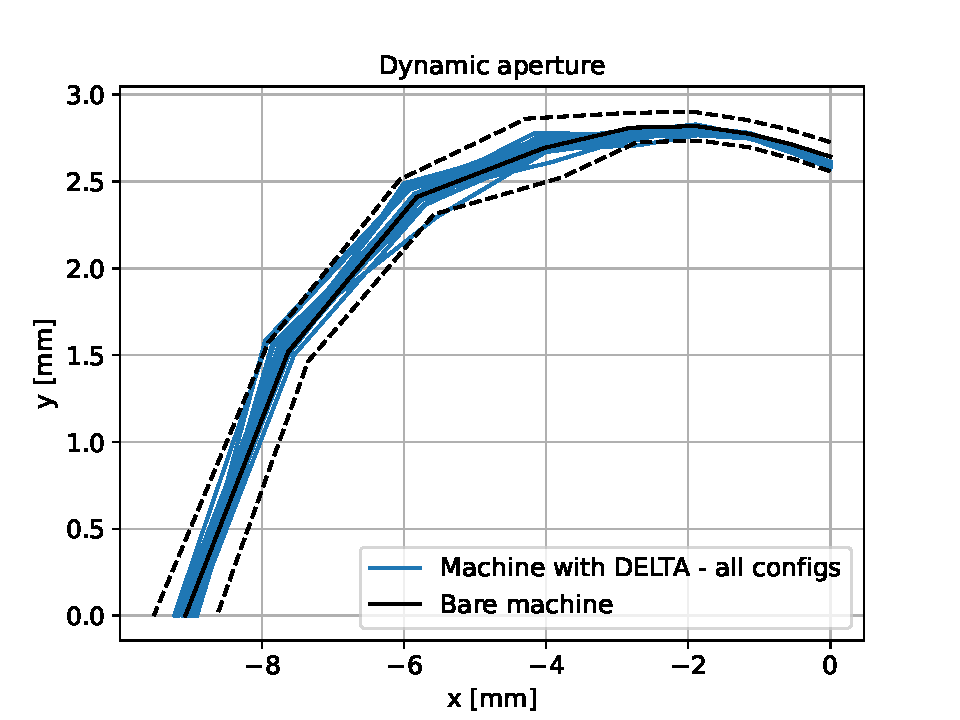
\includegraphics[width=.6\columnwidth]{THPS18_f1.pdf}
   \caption{Configuration space of DELTA52}
   \label{fig:config_space}
\end{figure}

\section{Effects on orbit}

To counteract the effects of the residual field integrals of the ID on the storage ring orbit, two corrector coils positioned adjacent to the ID operate in a FF scheme at an update rate of $\SI{10}{Hz}$. The FF table was calculated to compensate for the orbit distortions caused by each DELTA52 configuration.

The first step in calculating the FF table involved measuring orbit distortions for several ID configurations (approximately~\num{10} for each polarization line) with reference to its homing position ($K=0$, LH). Then, these distortions were filtered using the slow orbit feedback system (SOFB) response matrix (ORM) to compensate for orbit drifts due to other sources during the acquisitions. This process is accomplished by calculating the kicks of all SOFB correctors that best fit the horizontal and vertical measured orbit distortions, $\Delta\vec{r}$, then rebuilding them using only the SOFB correctors surrounding the DELTA52. We can express this process mathematically as:
\begin{equation}
    \Delta\vec{r}_\mathrm{f} = M_\text{S} P M_\text{S}^+\Delta\vec{r},
\end{equation}
where $M_\text{S} \in \mathbb{R}^{320\times281}$ is the SOFB ORM and $M_\text{S}^+$ its pseudo-inverse, $P \in \mathbb{R}^{281\times281}$ is a projection matrix that selects only the closest upstream and downstream horizontal and vertical correctors (in our case it was~\num{8} correctors in total),~\num{320} is the number of readouts of the~\num{160} BPMs and~\num{281} corresponds to all SOFB actuators,~\num{120}~HCMs,~\num{160}~VCMs plus the~RF frequency, and $\Delta\vec{r}_\mathrm{f}$ is the filtered orbit distortion, containing mainly the variation induced by the new ID position. These filtered distortions can be corrected using the FF CMs of the ID. The Jacobian of the FF correctors was calculated using the storage ring computer model, while  SOFB's ORM is the one routinely measured. The final stage involved interpolating the kicks for all~\num{5} polarization lines to ensure a smooth transition between adjacent measured configurations and continuity at the intersection of the lines. The employed solution was to create four 2D Gaussian process models~\cite{Gaussian} on the space depicted in Fig.~\ref{fig:config_space}, one for each FF CM strength. This model was finely sampled on each polarization line to create enlarged FF tables that were uploaded to the FF controller, where linear interpolation is used to define the corrector's strength at runtime.

Fig. \ref{fig:orbit_slow} illustrates the r.m.s of orbit distortions across all beam position monitors (BPMs) for various ID configurations with (dashed lines) and without (solid lines) the orbit FF acting. With FF-on,  the orbit residue is less than $\SI{2}{\mu m}$.%, which can be absorbed by the Fast Orbit Feedback System (FOFB) without saturation.

\begin{figure}[]
    \centering
   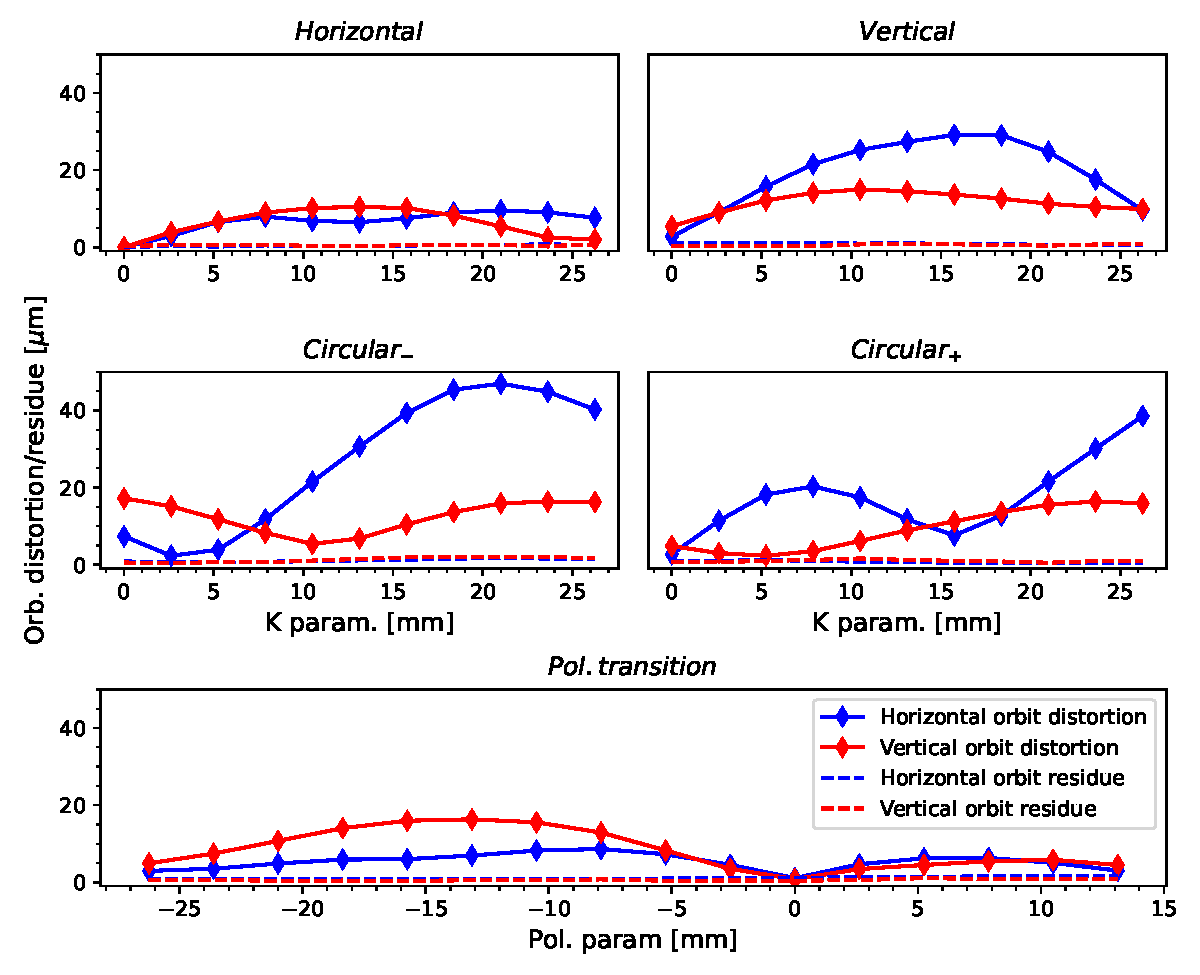
\includegraphics[width=0.9\columnwidth]{THPS18_f2.pdf}
   \caption{Effects of DELTA52 on orbit and residue of FF correction for all DELTA52 configurations}
   \label{fig:orbit_slow}
\end{figure}

In addition to statically characterizing orbit distortion and residual effects from FF compensation, the dynamic impact of device motion was assessed. An example of significant orbit distortion occurs for circular polarization with negative $K$ parameter variations ranging from $\SI{0}{mm}$ to $\SI{13.125}{mm}$, moving at a maximum speed of 1 mm/s. Fig. \ref{fig:orbit_fast} displays the r.m.s of the orbit distortion across all BPMs. The figure illustrates that FF compensation also effectively mitigates dynamic distortions from ID movement.

\begin{figure}[]
    \centering
   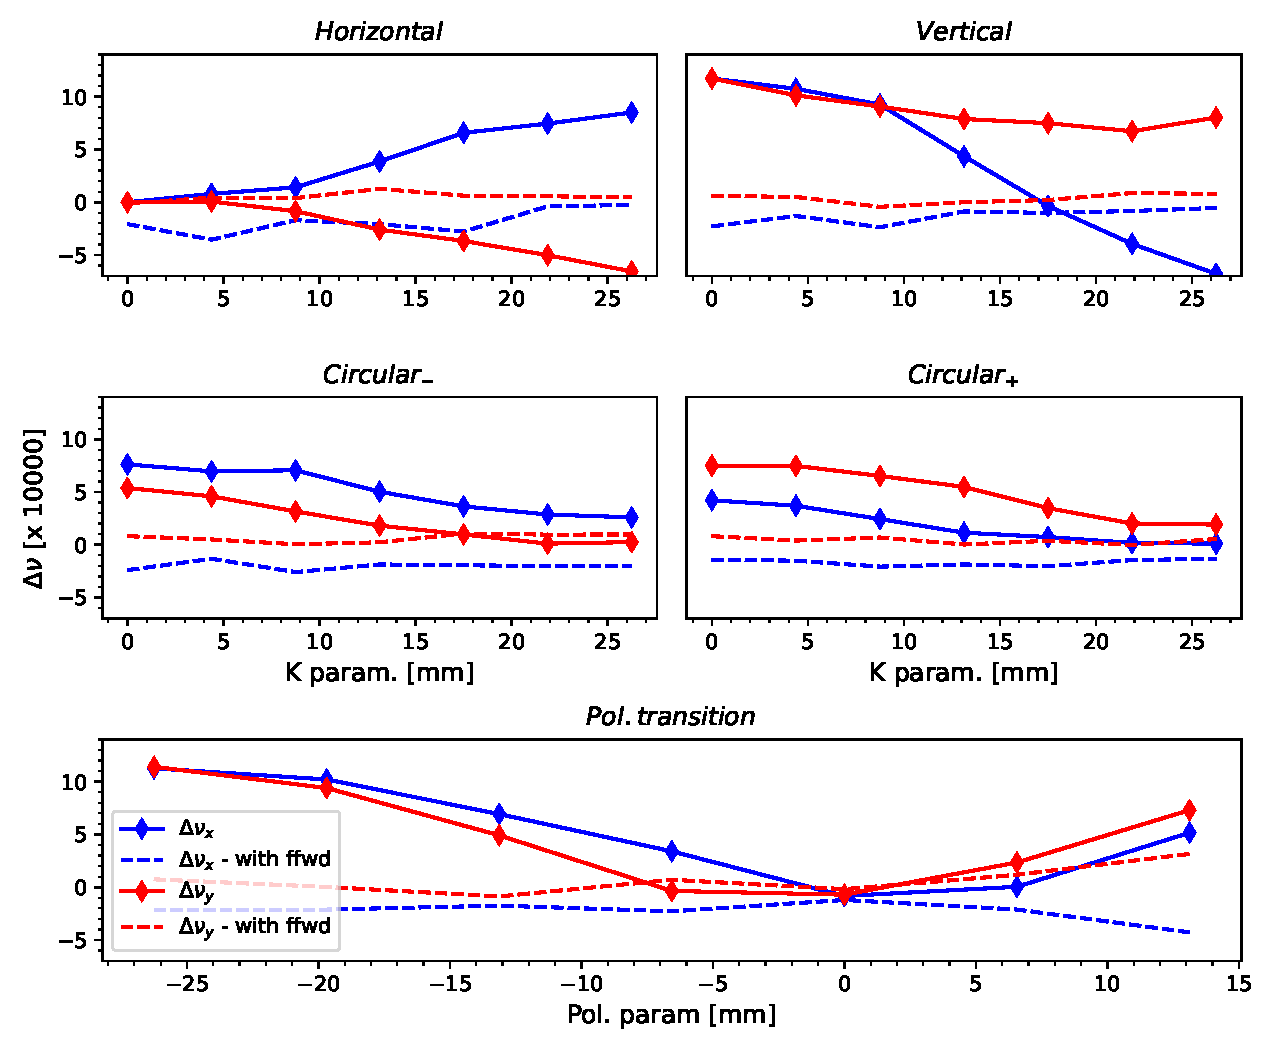
\includegraphics[width=0.68\columnwidth]{THPS18_f3.pdf}
   \caption{Effects of ID movimentation on orbit and FF compensation. The plot shows the r.m.s of the orbit distortion across all BPMs.}
   \label{fig:orbit_fast}
\end{figure}

\section{Effects on optics}

The effect of DELTA52 on the linear optics was also measured despite being very small. The betatron tune shifts as a function of the device configuration can be seen in Fig. \ref{fig:tunes}, where it is observed a tune shift of only 0.0012 in the worst-case.

\begin{figure}[]
    \centering
   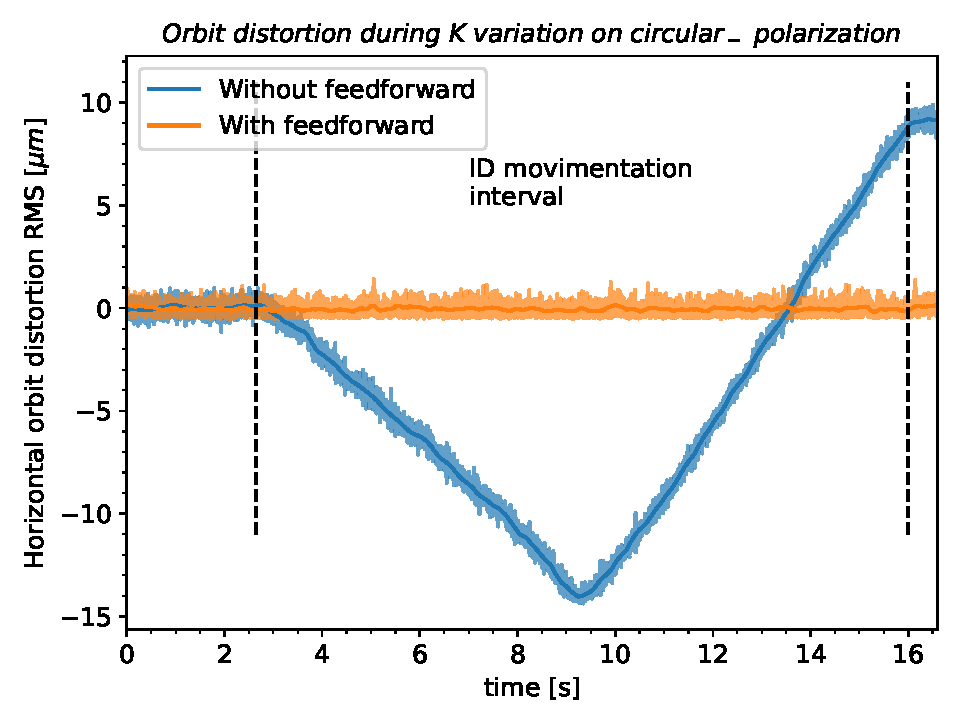
\includegraphics[width=0.9\columnwidth]{THPS18_f4.pdf}
   \caption{Effects of DELTA52 on tunes with and without FF.}
   \label{fig:tunes}
\end{figure}

Two methods have been employed to compensate for the impact on linear optics. The initial approach involves measuring the SOFB ORM for each DELTA52 configuration and subsequently minimizing the square of the difference between them and the matrix measured at the homing position, by adjusting the lattice quadrupole triplets located immediately upstream and downstream of the ID's straight section. Here, each matrix measurement took about ~\SI{3}{\minute} thanks to the use of the fast ORM measurement algorithm described in \cite{Velloso:IPAC22-MOPOTK002}. This method proved ineffective due to the small perturbation of the ID on optics, as the matrix measurements do not have enough sensibility to capture these effects.

The other approach only corrects the tune shifts by adjusting the same quadrupoles from the previous method. In this approach, the Jacobian describing the influence of quadrupole strengths on the tunes was measured. As the quadrupoles are adjusted symmetrically, this Jacobian forms a $2 \times 3$ matrix. The efficacy of this correction method is illustrated in Fig. \ref{fig:tunes}, indicating that the tune shifts were reduced to a variation range of less than~\num{0.0004}. This was achieved with very small adjustments of quadrupole strengths, below~\SI{0.07}{\percent}.

The impact of DELTA52 on coupling was also characterized and corrected. This correction method mirrored the initial approach tested for uncoupled optics. However, in this case, the objective was to minimize differences in the off-diagonal terms of the ORMs. This was achieved by adjusting the strength of the FF skew quadrupoles. For a non-invasive coupling estimation, the measured ORMs were utilized as inputs for the LOCO algorithm~\cite{Safranek} to calibrate the storage ring model. Subsequently, employing this model, the figure of merit used to estimate the coupling was the minimum tune separation. Fig.~\ref{fig:coupling} illustrates the difference in coupling with and without the actuation of skew quadrupoles FF. It's evident that FF implementation mitigates coupling variation across the $K$ parameters. Similar to the FF for orbit corrections, a Gaussian model was employed to interpolate skew strengths for all possible configurations.
 
\begin{figure}[]
    \centering
   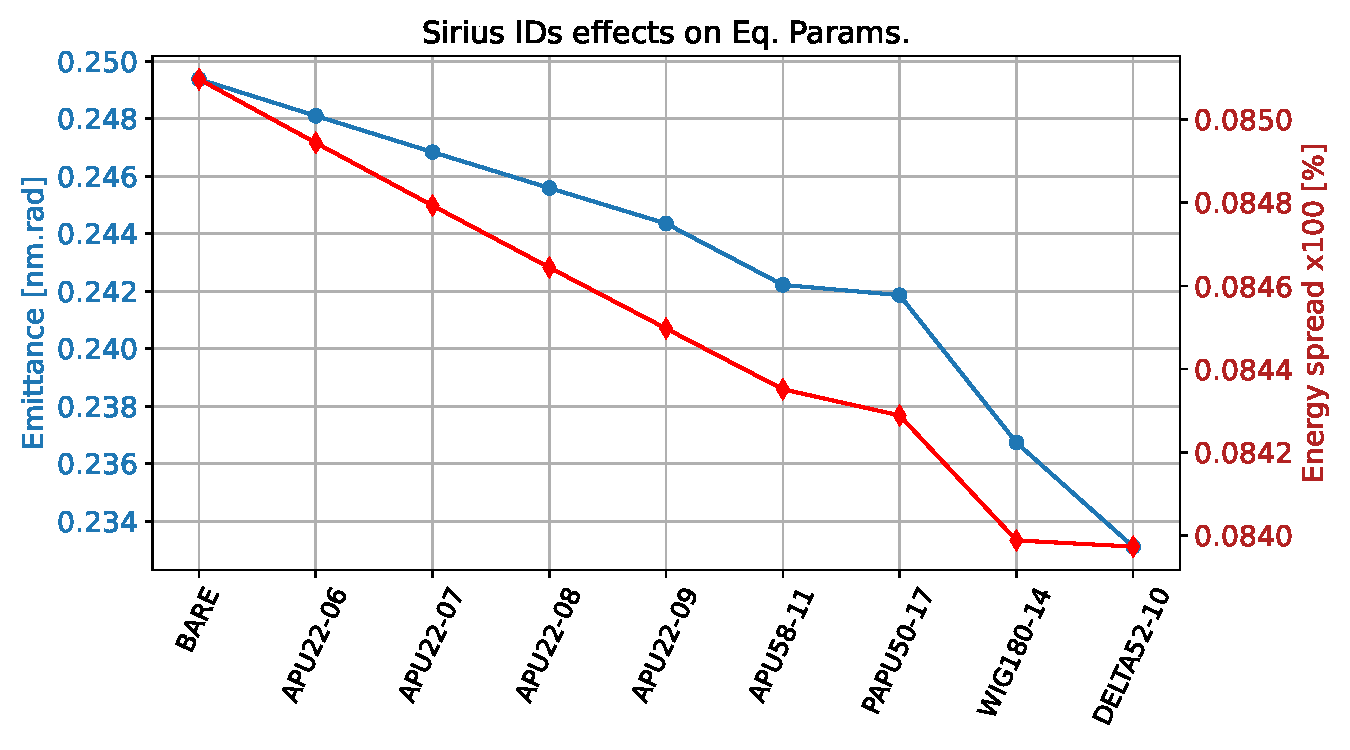
\includegraphics[width=.88\columnwidth]{THPS18_f5.pdf}
   \caption{Effects of DELTA52 on coupling with and without FF. The minimum tune separation was estimated by fitted models.}
   \label{fig:coupling}
\end{figure}


\section{Dynamic aperture}

Following the DELTA52 installation, no impact was noted on the off-axis injection efficiency. This confirmed the expectation from tracking simulations on machines with random errors. These simulations were executed using Trackcpp \cite{Trackcpp}, where the measured ID fields were modeled as kickmaps. Dynamic aperture (DA) calculations were performed for each ID configuration across 20 machines with random errors. The results of these calculations are shown in Fig. \ref{fig:dynapt}. In this figure, the solid lines represent the average DA for each ID configuration or bare machine, while the dashed lines represent the average DA $+/-$ the r.m.s.


\begin{figure}[]
    \centering
   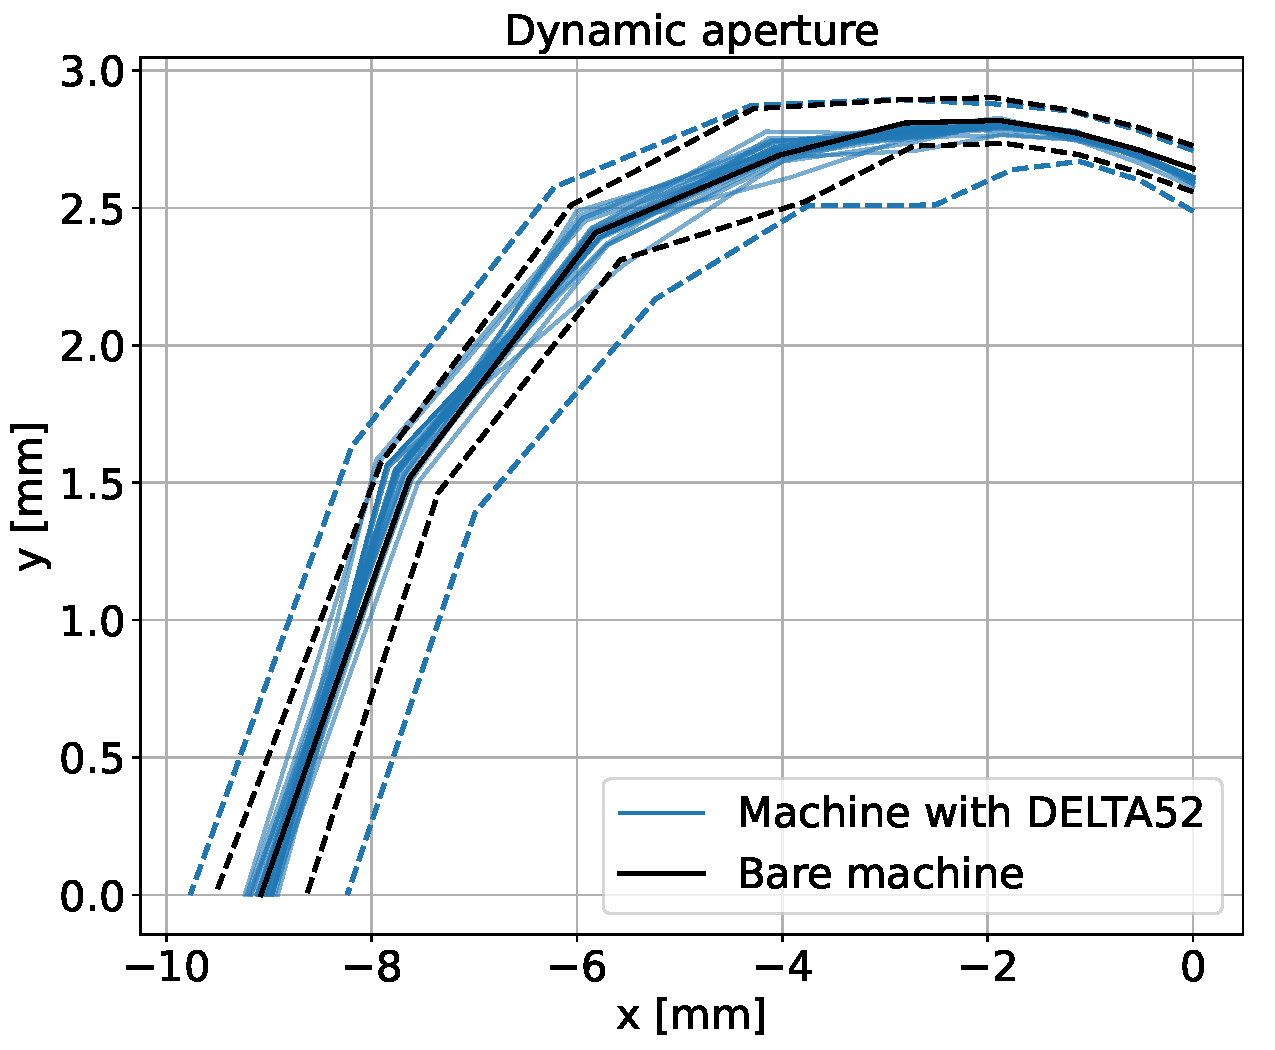
\includegraphics[width=0.6\columnwidth]{THPS18_f6.pdf}
   \caption{Impact of DELTA52 on dynamic aperture: Solid lines depict the average  DA across the 20 machines, whereas dashed lines illustrate the average DA $+/-$ the r.m.s.}
   \label{fig:dynapt}
\end{figure}

\section{Equilibrium parameters}
The influence on beam emittance and energy spread resulting from the inclusion of the ID was calculated using analytical expressions derived from synchrotron radiation integrals \cite{Lee:1999} and has not been yet characterized in the machine. Fig. \ref{fig:eq_param} shows the effect of all SIRIUS current IDs on the equilibrium parameters. In this calculation, it was assumed that all IDs were set to their maximum field configuration.

\begin{figure}[]
    \centering
   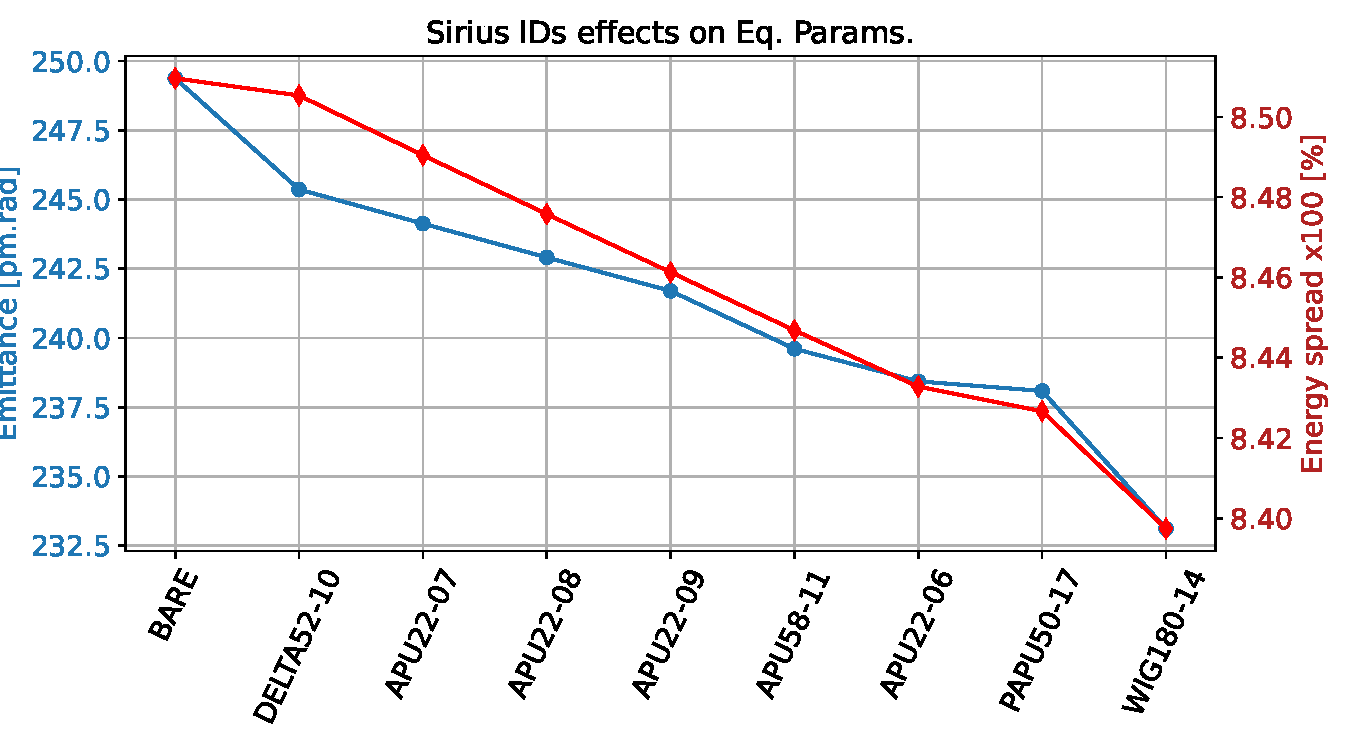
\includegraphics[width=.9\columnwidth]{THPS18_f7.pdf}
   \caption{Effects of SIRIUS IDs on equilibrium parameters. Calculations were made using analytical expressions from radiation integrals.}
   \label{fig:eq_param}
\end{figure}

The impact of DELTA52 on emittance is small, here it is worth remembering that the ID was placed in a straight section, where there is zero dispersion, which contributes to the reduction in emittance. Also, the DELTA52 introduces almost no effect on energy spread.

\section{CONCLUSIONS}

The results presented in this study indicate that the effects of the DELTA52 (installed in the SIRIUS low-$\beta$ straight section) are not prejudicial to the beam dynamics. Orbit distortions can be effectively corrected using the local FF system. Tunes are minimally affected, and thus, a FF correction is not a priority with the presently installed IDs. Nevertheless, employing a system using adjacent quadrupoles was demonstrated to reduce tune shifts by a factor of 3. Additionally, coupling correction using local skew quadrupoles has been shown to be effective. As for nonlinear effects, it was demonstrated that the dynamic aperture did not deteriorate, as evidenced by sustained good off-axis injection efficiency post-ID installation.
Finally, it was also shown by simulation methods that this new ID has a small impact on the equilibrium parameters. 

\section{ACKNOWLEDGEMENTS}
The authors thank the CNPEM Magnetic Systems Group (SMA) for providing field measurements and assistance with questions regarding the DELTA52.

\begin{thebibliography}{14} % Use for 1-9 references

%\cite{Liu:IPAC23-WEOGA2}
\bibitem{Liu:IPAC23-WEOGA2}
   L. Liu \emph{et al.},
   \textquotedblleft{Status of SIRIUS operation with users}\textquotedblright,
   in \emph{Proc. IPAC’23}, Venice, Italy, May 2023, pp. 2586--2589.
   \url{doi:10.18429/JACoW-IPAC2023-WEOGA2}    
    
    % \bibitem{Wiedemann:2015}
    %     Wiedemann, Helmut,
    %     \textquotedblleft{Overview of Synchrotron Radiation}\textquotedblright,
    %     in \emph{Particle Accelerator Physics}, Berlin Heidelberg, Germany: Springer, 2007, pp. 749-788.

\bibitem{Beamlines}
    LNLS,
    \textquotedblleft{SIRIUS Beamlines}\textquotedblright,
    available at https://lnls.cnpem.br/beamlines/

\bibitem{Vilela:IPAC17-WEPIK053}
    L. N. P. Vilela \emph{et al.},
    \textquotedblleft{Studies of DELTA-Type Undulators for Sirius}\textquotedblright,
    in \emph{Proc. IPAC’17}, Copenhagen, Denmark, May 2017, pp. 3045--3047.
    \url{doi:10.18429/JACoW-IPAC2017-WEPIK053} 
    
    %\cite{Vilela:IPAC18-TUPMK003}
\bibitem{Vilela:IPAC18-TUPMK003}
   L. N. P. Vilela, R. Basilio, J. F. Citadini, J. R. Furaer, and F. Rodrigues,
   \textquotedblleft{Advances in the Sirius DELTA-Type Undulator Project}\textquotedblright,
   in \emph{Proc. IPAC’18}, Vancouver, Canada, Apr.-May 2018, pp. 1491--1493.
   \url{doi:10.18429/JACoW-IPAC2018-TUPMK003}  

    %\cite{Ascenção:IPAC23-MOPM088}
\bibitem{Ascenção:IPAC23-MOPM088}
   G. Ascenção, M. Alves, L. Liu, and X. Resende,
   \textquotedblleft{Study of insertion devices effects in SIRIUS}\textquotedblright,
   in \emph{Proc. IPAC’23}, Venice, Italy, May 2023, pp. 1184--1187.
   \url{doi:10.18429/JACoW-IPAC2023-MOPM088}    

 \bibitem{Gaussian}
    Liu, Miao \emph{et al.},  
    \textquotedblleft{Gaussian Processes for Learning and Control: A Tutorial with Examples}\textquotedblright,\emph{IEEE Control Systems}, vol. 38, no. 5, 2018, pp. 53–86.
    \url{doi:10.1109/MCS.2018.2851010. }

\bibitem{Velloso:IPAC22-MOPOTK002}
   M. M. S. Velloso, M. B. Alves, and F. H. de Sá,
   \textquotedblleft{Fast Orbit Response Matrix Measurement via Sine-Wave Excitation of Correctors at Sirius}\textquotedblright,
   in \emph{Proc. IPAC’22}, Bangkok, Thailand, Jun. 2022, pp. 425--428.
   \url{doi:10.18429/JACoW-IPAC2022-MOPOTK002}  
   
\bibitem{Safranek}
	 J. Safranek,
		\textquotedblleft{Experimental determination of storage ring optics using orbit response measurements}\textquotedblright,
		\emph{Nucl.  Instr. Meth. A}, vol 388, pp.27--36, 1997.
        \url{doi:10.1016/S0168-9002(97)00309-4}

\bibitem{Trackcpp}
    LNLS Accelerator Physics Group,
    \textquotedblleft{Tracking library}\textquotedblright,
    available at https://github.com/lnls-fac/trackcpp
        
\bibitem{Lee:1999}
    S. Y.Lee,
    \textquotedblleft{Physics of Electron Storage Rings}\textquotedblright,
    in \emph{Accelerator physics}, London, UK: World Scientific, 1999, pp. 383-458.

 






%    \bibitem{Liu:2015jpo}
%        L. Liu, N. Milas, A. Mukai, X. Resende and F. de Sá,
%        \textquotedblleft{Upgraded Optics for Sirius With Improved Matching of Electron and Photon Beam Emittances}
%        \url{doi:10.18429/JACoW-IPAC2015-TUPWA007}
        
%    \bibitem{Liu:IPAC2016-THPMR011}
%        L. Liu, X.R. Resende, A.R.D. Rodrigues, F. H. de Sá,
%       \textquotedblleft{{I}njection {D}ynamics for {S}irius {U}sing a {N}onlinear {K}icker}\textquotedblright,
%       in \emph{Proc. IPAC’16}, Busan, Korea, May 2016, pp. 3406--3408.
%       \url{doi:10.18429/JACoW-IPAC2016-THPMR011} 
 
%    \bibitem{deSá:IPAC2016-THPMR012}
%        F. H. de Sá, L. Liu, X.R. Resende,
%       \textquotedblleft{{O}ptimization of {N}onlinear {D}ynamics for {S}irius}\textquotedblright,
%       in \emph{Proc. IPAC’16}, Busan, Korea, May 2016, pp. 3409--3412.
%       \url{doi:10.18429/JACoW-IPAC2016-THPMR012}       
       
%	\bibitem{Huang:2013}
%		X. Huang, J. Corbett, J. Safranek, J. Wu,
%		\textquotedblleft{An algorithm for online optimization of accelerators}\textquotedblright,
%		\emph{Nucl.  Instr. Meth.}, vol 726, pp. 77--83, 2013.
%        \url{https://doi.org/10.1016/j.nima.2013.05.046} 

%    \bibitem{Huang:2015}
%		X. Huang, J. Safranek,
%		\textquotedblleft{Online optimization of storage ring nonlinear beam dynamics}\textquotedblright,
%		\emph{Phys. Rev. ST Accel. Beams}, vol 18, p. 18, .
%        \url{10.1103/PhysRevSTAB.18.084001} 
 
%    \bibitem{Liuzzo:IPAC2016-THPMR015}
%        S.M. Liuzzo, \emph{et al.},
%        \textquotedblleft{RCDS Optimizations for the ESRF Storage Ring}\textquotedblright,
%        in \emph{Proc. IPAC’16}, Busan, Korea, May 2016, pp. 3420--3423.
%       \url{doi:10.18429/JACoW-IPAC2016-THPMR015}   
    
%    \bibitem{Olsson:IPAC2018-WEPAL047}
%       D.K. Olsson,
%       \textquotedblleft{Online Optimisation of the MAX IV 3 GeV Ring Dynamic Aperture}\textquotedblright,
%       in \emph{Proc. IPAC'18}, Vancouver, BC, Canada, Apr. 4,, pp. 2281--2283,
%       \url{doi:10.18429/JACoW-IPAC2018-WEPAL047}

    
%    \bibitem{yang:ipac2022-tupopt064}
%        X. Yang,\emph{et al.},
%       \textquotedblleft{Online Optimization of NSLS-II Dynamic Aperture and Injection Transient}\textquotedblright,
%        in \emph{Proc. IPAC'22}, Bangkok, Thailand, Jun. 2022, pp. 1159--1162.

%       \url{doi:10.18429/JACoW-IPAC2022-TUPOPT064}
    
   
	\end{thebibliography}


\end{document}
